\subsection{Summary of Work}
The objective of this work is to identify the existence probability of a semi-orthogonal user selection group as a function of SNR and SIR requirements, group size, number of transmit antennas, and the number of users or stations (STAs) considered as candidates for addition to the semi-orthogonal user selection group. 

The rate of growing the number of users considered vs. increasing the SNR requirements is also investigated asymptotically.

\subsection{SNR ad SIR Requirements}
The requirement for a $\epsilon$-orthogonal group (semi-orthogonal user selection group, or SUS group) is broken into two parts. Firstly the users in the group are required to have a channel norm similar to other users in the group. The upper and lower bound on SNR ensures that users in an SUS group have similar channel gains. Asserting an upper and lower bound can be viewed a coarse form of power control. The upper and lower bound can be adjusted to a narrow improving linear precoding or fine power control performance. Since the norms of the channels in the SUS group are similar, the precoding weights should also be similar, allowing for more even distribution of weights between precoding factors.

The second requirement deals with interference between users in an SUS group. Once it has been determined that a given user meets the SNR requirement, then it is compared against other candidate users to ensure interference is sufficiently low. The inner product between a user's channel and other candidate user's channels is formed. The magnitude of the product is compared to some threshold , $\epsilon$. If the product is lower than the threshold, users are said to be $\epsilon$-orthogonal and the users are added to the SUS group.

The expression for a SUS group requirements is given by as:

\begin{equation}\label{eq:S_e}
    \begin{aligned}
        \mathcal{S}_\epsilon = \lbrace \mathcal{S}_a \big|\ | \textbf{h}_i\textbf{h}_j^H |\ <\ \epsilon \ \text{;} \ \rho^-<\Vert \textbf{h}_i \Vert^2 < \rho^+\ \forall \ i \neq j \in \mathcal{S}_a \rbrace
    \end{aligned}
\end{equation}

\subsection{Existence Probability of SUS Groups}
The main contribution of the work is to develop an expression for the existence probability of an SUS group. Swannack develops a lower bound on the existence probability, $Pr[\mathcal{S}_\epsilon \neq \lbrace \emptyset \rbrace]$. Probability of SUS group existence depends on the orthogonality requirements given in Eq. (\ref{eq:S_e}), the group size $l = \vert \mathcal{S}_a \vert$, and the number of candidate users considered for addition to the SUS group, $n$. 

Swannack considers an example to illustrate results. The example is shown in Fig. \ref{fig:swannack_fig5a}, this example was replicated with results of replication shown in Fig. \ref{fig:reproduce_fig5a}. The purpose of this example is to determine the number of users that must be evaluated for addition to an SUS group of size 2, 3, and 4 to achieve a probability of existence of 90\%. In this example 4 transmit antennas are assumed.

\begin{figure}
    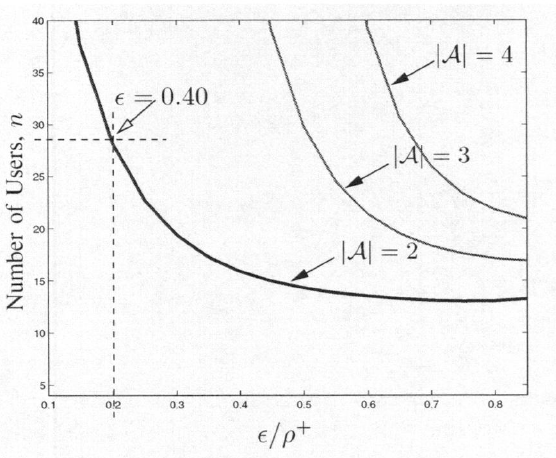
\includegraphics[width=12cm]{figs/swannack_fig5a.png}\\
    \caption{Plot of minimum number of users to achieve minimum probability of SUS group existence of 0.9. 4 transmit antennas are assumed for all curves.}
    \label{fig:swannack_fig5a}
\end{figure}

\begin{figure}
    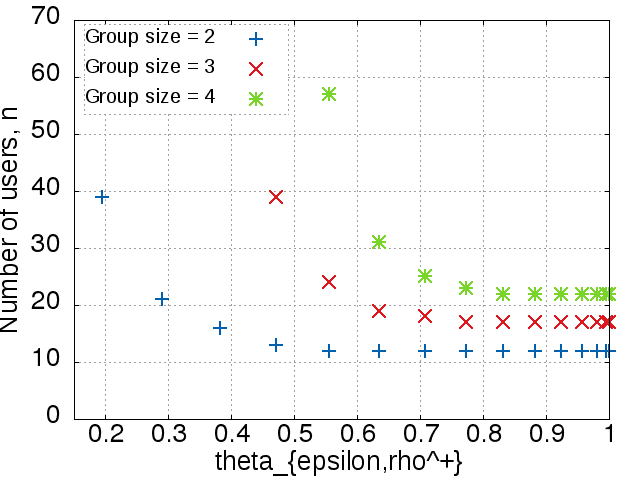
\includegraphics[width=12cm]{figs/existence.png}\\
    \caption{Plot of minimum number of users to achieve minimum probability of SUS group existence of 0.9. 4 transmit antennas are assumed for all curves. Horizontal axis scale is $\cos{(\theta_\epsilon,\rho^+)} = \frac{\epsilon}{\rho^+}$}
    \label{fig:reproduce_fig5a}
\end{figure}

The results shown in Fig. \ref{fig:swannack_fig5a} are developed a geometric interpretation. The geometric interpretation developed by Swannack involves projecting channel onto the surface of complex $m$-dimensional sphere (where $m$ is analogous to the number of transmit antennas), then considering probability of overlapping spherical caps in this space. The gometric model is split into two parts: the SNR requirement, and this SIR (orthogonality) requirement.

The geometric analog of user $i$'s channel, $\textbf{h}_i$, satisfying the SNR requirement is that $\Vert\textbf{h}_i\Vert^2$ lies in the real spherical 2$m$ shell between $\rho^-$ and $\rho^+$. The geometric analog of the orthogonality requirement is that the angle formed between any two channels in the SUS group are greater than $\arccos{(\frac{\epsilon}{\rho^+})}$. First we consider SNR requirement developed by Swannack.

In the complex-channel case presented by Swannack, the probability that the channel satisfies SNR requirements is given by:
\begin{equation}\label{eq:p_s}
    \begin{aligned}
        p_s = \Gamma_n(2m,m\rho^-) - \Gamma_n(2m,m\rho^+)
    \end{aligned}
\end{equation}

The above expression assumes that $\textbf{h}_i$ is a circularly symmetric Gaussian random variable with zero mean and variance  $\frac{1}{2m}$. Therefore the L2 norm of the channel will follow a Chi-squared distribution with $\vert \mathcal{S}_a\vert$ degrees of freedom (ie. size of the SUS group). The above expression also assumes that the SUS group size is equal to the number of transmit antennas, m: $\vert \mathcal{S}_a\vert = m$. Note that the incomplete gamma function in (\ref{eq:p_s}) are assumed to be normalized. A more detailed description of the derivation of this equation will be discussed in the following aside. Resulting comments from the discussion will then be related back to this expression.\\
\underline{\textbf{Aside: derivation and notes regarding Eq. (\ref{eq:p_s})}:}

 Given a standard normal random variable, $X_k\sim\mathcal{N}(0,1)$, corresponding realization, $x_k$, probability density function (PDF) $f_Xk(x_k)$, and cumulative distribution function (CDF) $F_Xk(x_k)$:

\begin{equation}\label{eq:normal}
    \begin{aligned}
        f_Xk(x_k) &= \frac{1}{\sqrt{2\pi}}e^{-\frac{x_k^2}{2}}\\
        F_Xk(x_k) &=\frac{1}{2}(1+\text{erf}(\frac{x_k}{\sqrt{2}}))
    \end{aligned}
\end{equation}

Let $\textbf{X}$ denote an iid vector of length $K$. Each element of $\textbf{X}$ follows the standard normal distribution given in Eq. (\ref{eq:normal}, that is, $X_i\in\textbf{X}\ \forall i = 1,2\ldots K$.

Let $Y$ be the random variable representing the L2 norm of the vector $\textbf{X}$:
\begin{equation}\label{eq:ch_sq_sum}
    \begin{aligned}
        Y &= \Vert \textbf{X} \Vert^2\\
          &= \sum_{k = 1}^K X_kX_k^*
    \end{aligned}
\end{equation}

It is well-known that a K-length sum of square standard normal random variables results in a Chi-squared distribution.The PDF and CDF of the Chi-squared distribution associated with $Y$ in terms of realizations $y = \sum_{k=0}^K x_k x_k^*$ are given by $f_Y(K,y)$, and $F_Y(K,y)$, respectively:
\begin{equation}\label{eq:ch_sq}
    \begin{aligned}
        f_Y(K,y) &= \frac{1}{2^{K/2}\Gamma(K/2)}y^{\frac{K-2}{2}}e^{\frac{-y}{2}};\\
        F_Y(K,y) &= \frac{\gamma(K/2,y/2)}{\Gamma(K/2)}\\
        &= \Gamma_n(K/2,y/2)
    \end{aligned}
\end{equation}

Now we wish to investigate the case where the normal distributions are no longer standard. Rather, they are zero-mean normal distributions with variance $\sigma^2$. Let $Z$ denote the scaled sum:
\begin{equation}\label{eq:ch_sq_sum_scaled}
    \begin{aligned}
        Z &= \Vert \sigma \textbf{X} \Vert^2\\
          &= \sigma^2 \sum_{k = 1}^K X_kX_k^*
    \end{aligned}
\end{equation}

Therefore the associated PDF and CDF become:
\begin{equation}\label{eq:ch_sq_scaled}
    \begin{aligned}
        f_Z(K,z) &= \frac{1}{\sigma^{K/2}2^{K/2}\Gamma(K/2)}z^{\frac{K-2}{2}}e^{\frac{-z}{2\sigma^2}};\\
        F_Z(K,z) &= \Gamma_n(K/2,z/(2\sigma))
    \end{aligned}
\end{equation}
\underline{\textbf{(End aside)}}

Returning to the practical case at hand, we have  $\textbf{h}_i$ which is a circularly symmetric Gaussian random variable with zero mean and variance  $\frac{1}{2m}$. Recall that the length of this vector is the same as the number of transmit antennas, $m$. We can apply Eq. (\ref{eq:ch_sq_scaled}) from the aside discussion in order to develop an expression for the CDF of the channel norm. The CDF of the channel norm will be denoted by $F_{\Vert\textbf{hi}\Vert^2}(m,h_m)$, where $h_m$ are realizations of the random variable formed by the channel norm. 

Each term in the $m$-length vector, $\textbf{h}_i$ is represented by two normal random variables: one for the real part and one for the imaginary part. When forming the L2 norm of the $m$-length vector, each multiplication forms a sum of length four where each of the arguments of the sum are a product of two random variables. Namely, the sum takes the form real$\cdot$real + real$\cdot$imaginary + imaginary$\cdot$real+ complex$\cdot$complex. Even though this sum can be simplified to a complex number, each term in the sum adds a degree of freedom to the resulting Chi-squared distribution. Thus, when forming the CDF , the expression becomes:

\begin{equation}\label{eq:ch_sq_cdf_chan}
    \begin{aligned}
        F_{\Vert\textbf{hi}\Vert^2}(m,h_m) = \Gamma_n(2m/2,mx)
    \end{aligned}
\end{equation}

Now we turn our attention to Swannack's expression of probabilities associated with the orthogonality requirement, rather than the SNR requirement. Swannack develops a lower bound on the probability associated with the orthogonality constraint, $p_\perp$, as:
\begin{equation}\label{eq:p_perp}
    \begin{aligned}
        p_\perp \geq (1-(1-l)\delta_c(\theta_{\epsilon,\rho},2m))^{l-1}
    \end{aligned}
\end{equation}

The function $\delta_c(\theta,2m)$ is defined as the ratio of the area of a spherical (polar) caps of a sphere in $2m$ dimensions formed by $\theta$ to the entire surface area of the sphere:

\begin{equation}\label{eq:delta_c_sphere}
    \begin{aligned}
        \delta_c(\theta,2m) = 2\frac{\Omega_{2m}(\theta)}{\Omega_{2m}(\pi)}
    \end{aligned}
\end{equation}

Swannack develops upper and lower bounds on $\delta_c$ (TODO: elaborate on these bounds as necessary--will likely be required as we consider developing new bounds in the widely linear case).

Some investigation into the impact of change in number of dimensions on $\delta_c$ lower bounds are shown in Fig. \ref{fig:delta}.
\begin{figure}
    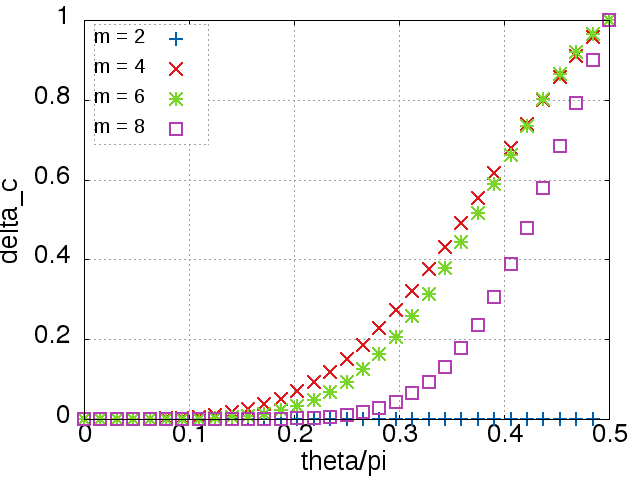
\includegraphics[width=12cm]{figs/delta.png}\\
    \caption{Plot of $\delta_c$ as a function of $\theta_{\epsilon,\rho}$ over various dimensions (ie. number of transmit antennas)}
    \label{fig:delta}
\end{figure}

Several additional plots investigating impact of changes in SUS group size and number of dimensions are shown in Figs. \ref{fig:p_orth_gs_2}, \ref{fig:p_orth_gs_4}, \ref{fig:p_orth_gs_6}, \ref{fig:p_orth_gs_8}.

\begin{figure}
    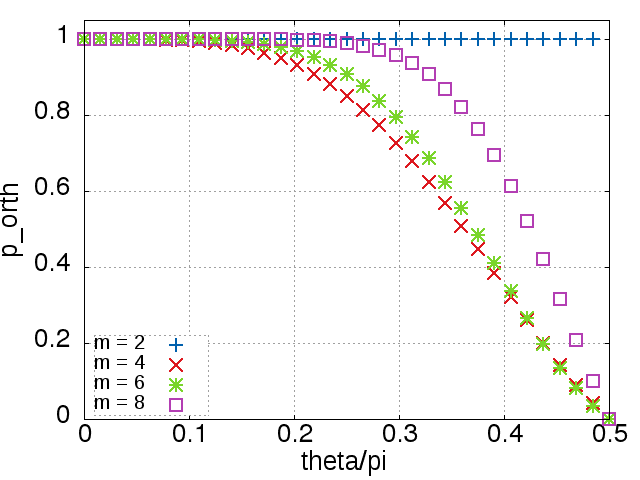
\includegraphics[width=12cm]{figs/p_orth_gs_2.png}\\
    \caption{Plot of $p_{\perp}$ as a function of $\theta_{\epsilon,\rho}$ over various dimensions (ie. number of transmit antennas), SUS group size of 2}
    \label{fig:p_orth_gs_2}
\end{figure}

\begin{figure}
    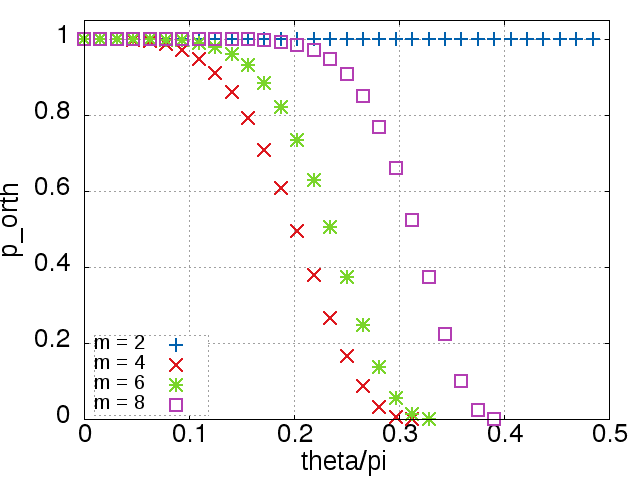
\includegraphics[width=12cm]{figs/p_orth_gs_4.png}\\
    \caption{Plot of $p{\perp}$ as a function of $\theta_{\epsilon,\rho}$ over various dimensions (ie. number of transmit antennas), SUS group size of 4}
    \label{fig:p_orth_gs_4}
\end{figure}

\begin{figure}
    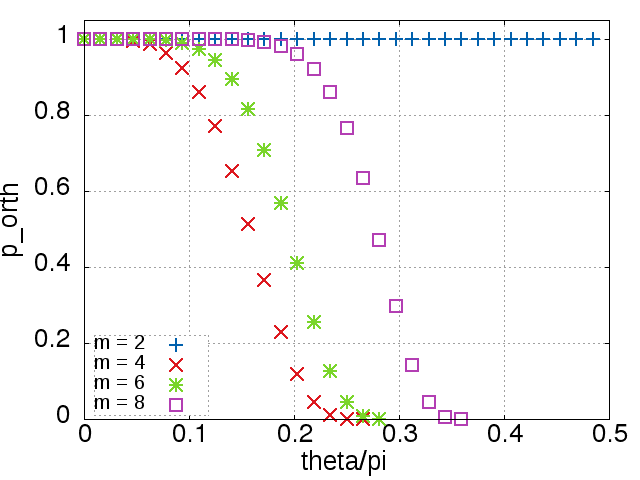
\includegraphics[width=12cm]{figs/p_orth_gs_6.png}\\
    \caption{Plot of $p{\perp}$ as a function of $\theta_{\epsilon,\rho}$ over various dimensions (ie. number of transmit antennas), SUS group size of 6}
    \label{fig:p_orth_gs_6}
\end{figure}

\begin{figure}
    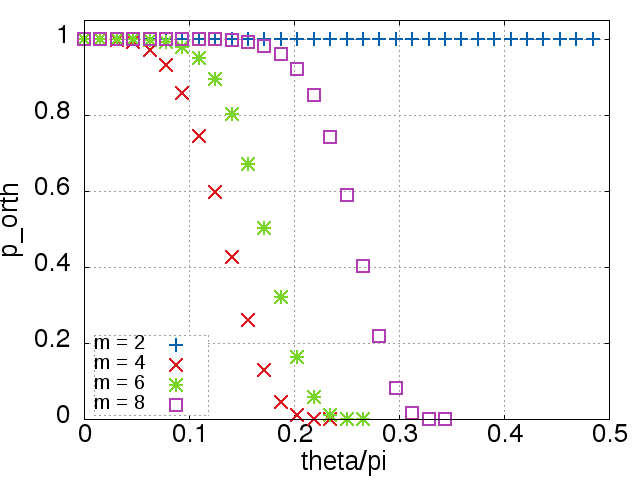
\includegraphics[width=12cm]{figs/p_orth_gs_8.png}\\
    \caption{Plot of $p{\perp}$ as a function of $\theta_{\epsilon,\rho}$ over various dimensions (ie. number of transmit antennas), SUS group size of 8}
    \label{fig:p_orth_gs_8}
\end{figure}

\newpage
\subsection{Extending results to relaxed, widely linear orthogonality constraint}

We now consider relaxing the orthogonality and SNR constraints, by limiting  requirements to only the real part of the channel inner product and norm. First we introduce the following definitions. Let the  transformation, $\mathcal{T}$, be the transformation of the complex vector in $\mathbb{C}^m$ to a real vector in $\mathbb{R}^{2m}$:
\begin{equation}\label{eq:complex_real_xform}
    \begin{aligned}
        \textbf{h}_i \in \mathbb{C}^m \xrightarrow{\mathcal{T}} \overline{\textbf{h}}_i = [ \mathfrak{Re} \lbrace \textbf{h}_i \rbrace \ \mathfrak{Im}\lbrace \textbf{h}_i \rbrace ] \in \mathbb{R}^{2m}
    \end{aligned}
\end{equation}
Thus,
\begin{equation}\label{eq:orth_real_transp}
    \begin{aligned}
        \mathfrak{Re} \lbrace \textbf{h}_i\textbf{h}_j^H \rbrace = \overline{\textbf{h}}_i \overline{\textbf{h}}_j^T 
    \end{aligned}
\end{equation}

Following from these definitions and Swannack's expression for SUS groups meeting SNR and orthogonality requirements, the relaxed expression for the collection of SUS groups becomes:
\begin{equation}\label{eq:wl_S_e}
    \begin{aligned}
        \mathcal{S}_\epsilon = \lbrace \mathcal{S}_a \big|\  \overline{\textbf{h}}_i \overline{\textbf{h}}_j^T<\ \epsilon \ \text{;} \ \rho^-<\Vert \overline{\textbf{h}}_i \Vert^2 < \rho^+\ \forall \ i \neq j \in \mathcal{S}_a \rbrace
    \end{aligned}
\end{equation}

The geometric model developed by Swannack is still useful in the relaxed widely linear case given in (\ref{eq:wl_S_e}). However, further discussion regarding expressions for relaxed $p_s$, $p_\perp$ is required.

The Chi-squared distribution used to derive the expression in (\ref{eq:p_s}), now only has 2$m$ degrees of freedom, rather than 4$m$ degrees of freedom. Therefore the expression for relaxed (widely linear) $p_s$ becomes:
\begin{equation}\label{eq:p_s_real}
    \begin{aligned}
        p_{s,wl} = \Gamma_n(m,m\rho^-) - \Gamma_n(m,m\rho^+)
    \end{aligned}
\end{equation}

